\Chapter{Képek közelítése a bemeneti vektorok terében}

A GAN által betanult térről nem kapunk egzakt információkat, nincs tudomásunk arról, hogy a modell hogyan helyezte el a sokdimenziós térben a tanult ismereteit. Egy betanított modell esetén csupán annyit látunk, hogy különböző random bemeneti vektorokra különféle képeket kapunk a generátor kimenetén.
Két random zajvektor között ha interpolálunk, akkor minden egyes mintavételezett pontból ki tudunk generálni olyan képeket, amelyek a két kép közti átmenetet jelentik és amelyeken megfigyelhetőek a két kép együttes tulajdonságai. A \ref{fig:interpolation} ábrán látható egy példa az interpolációra.

\begin{figure}[h]
\centering
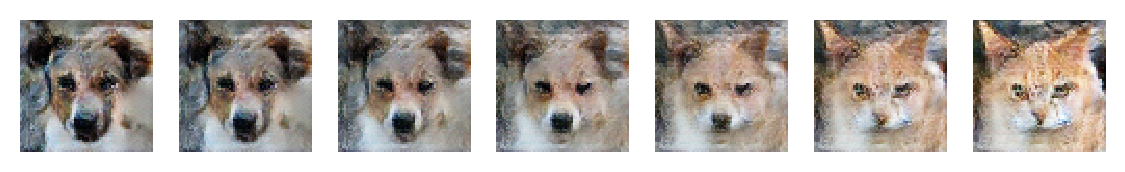
\includegraphics[width=15cm]{images/interpolation.png}
\caption{Generált képek lineáris interpolációval két zajvektor között}
\label{fig:interpolation}
\end{figure}

A bemeneti vektorok teréről feltételezhetjük, hogy folytonosan van kitöltve, mivel bármely pontra egy képet kaphatunk vissza. Viszont ezen tér feltérképezése sem egy triviális feladat és az sem biztosított, hogy a talált pont környezetéből mintavételezve hasonló tulajdonságú képek generálhatóak ki.

A GAN tanítása során a generátor a bemeneti vektorok terére megtanulja, hogy a tér egyes pontjaira milyen adatot képezzen le. A térből mintavételezett adatok mindegyikére egy, a tanítóhalmaz eloszlását követő adatot tud kigenerálni.
A tanítási lépések során általában a Normális vagy Egyenletes eloszlás szerint generálunk pontokat és azok alapján tanul a generátor modellünk. Annak ellenére, hogy a tér egyes pontjaira igen jól betanul a modell, nem garantálható, hogy az így keletkezett tér megfelelően klaszterezhető lehet és valójában a tanítás során generált pontok eloszlását követik a klaszterek pontjai \cite{mukherjee2019clustergan}.

\Section{Képek közelítése pixel-szinten}
A képek közelítésre egy megoldás lehet a \textit{synthesis-through-optimization}\cite{frans2021clipdraw} technika, amelyhez nem kell betanítani egy újabb modellt, csupán optimalizációs alapon történik meg a képek közelítése.
A technika megvalósításához szükségünk van egy olyan függvényre, amely adott bemenetre egy várt kimenetet generál, ez esetünkben a Generátor modell. Az bemenetre kapott kimenetet ezután meg kell vizsgálni és egy célfüggvény segítségével ki kell értékelni, majd a hibaérték alapján módosítani kell a bemenetet olyan irányba, hogy a hiba csökkenjen.

A kimenet vizsgálatára általában egy osztályozót szokás alkalmazni, a következő alfejezetben az a módszer kerül majd bemutatásra. Viszont a bemenet optimalizálási módszere egy egyszerűbb vizsgálati stratégia mellett kerül bemutatásra az érthetőség növelése érdekében.

%TODO: A jelölések egységesítése! (nem csak erre az alfejezetre vonatkozólag!)
A GAN $G$ generátorának bemenete egy $\vec{z} \in \mathbb{R}^{z_n}$ vektor, ahol $z_n$ általában 100 szokott lenni. Vagyis a bemeneti vektor egy $z_n$ dimenziójú tér egy pontja. A 100 dimenzióban történő keresés igen nehéz lehet a hagyományos heurisztikus módszerekkel, mint például a hegymászó módszerrel. A hegymászó optimalizáló módszer során a célfüggvényt minimalizáljuk (vagy maximalizáljuk) a pont körüli tartomány mintavételezésével, majd a megfelelő szomszédos pontra való lépéssel. A bemeneti paraméter lehet a pont kiinduló pozíciója, a lépésköz és a mintavételezés sűrűsége. A megfelelő pontosság érdekében igen sok mintára lehet szükségünk és ez egy sokdimenziós térben igen sok minta szükséges a tér feltérképezésére. A fix lépésköz és a mintavételezés pontatlanságának hatására könnyedén lokális optimumokban ragadhat az algoritmus. Több vizsgálandó pont elszórása a térben megnövelheti az esélyét annak, hogy rátalálunk a globális optimumra is, viszont ez jelentősen megnöveli a számításigényt.
A gradiens módszer vagy gradiens-süllyesztés (\textit{Gradient Descent}) egy olyan iteratív optimalizáló módszer, amely a differenciálható függvény lokális minimumának megtalására irányul. A célfüggvény elsőrendű deriváltjai igazítják el a vizsgált pontunkat a minimumhoz. \cite{ruder2016overview}

Két kép között a pixelszintű távolságot az L2 norma vagy euklideszi norma segítségével kaphatjuk meg.

$$ \|x\|_2 = \left({\sum_{i=1}^{n}|x_i|^2}\right)^{\frac{1}{2}} $$

Egy kiválasztott kép közelítése a bemeneti vektorok terében az alábbi módon történhet:\\ 
Jelölje $X$ a keresendő képet, $G$ a generátort, $\vec{z} \in \mathbb{R}^{z_n}$ pedig a látens vektort.\\
A cél egy olyan $\vec{z} \in \mathbb{R}^{z_n}$ látens vektor keresése, amellyel az alábbi távolság minimalizálható.

$$ \min\left(\sum_{i=1}^{n\times m}\sqrt{(X_i-G(\vec{z})_i)^2}\right)$$

A képeket tehát pixelszinten hasonlítjuk össze kiindulásképp. Ez a távolságot szokás L2 távolságnak is nevezni, az L2 norma alapján, vagy euklideszi távolságnak is.
Egyéb metrikákat is alkalmazhatunk a képek hasonlóságának mérésére, ilyen a PCA, a HOG, MSE, stb...

Legyen $l$ a lépésméret, $X \in \mathbb{R}^{n\times m \times 3}$ a keresendő kép, $G$ pedig a betanított generátor.
\begin{enumerate}
	\item Generáljunk egy képet az aktuális $\vec{z}$ zajvektorral
$$\hat X = G(\vec{z})$$
	\item Számoljuk ki a generált kép és a keresendő kép távolságát.
$$ loss = \sum_{i=1}^{n\times m}\sqrt{(X_i-\hat X_i)^2} $$
	\item Számoljuk ki a gradienseket a hibafüggvény szerint
$$ \vec{grad} = \frac{d}{d\vec{z}} \left[loss\right]$$
	\item Módosítsuk a $\vec{z}$ zajvektor elemeit a kapott gradiensek szerint egy $l$ hosszúságú lépéssel
$$ z_i = z_i - (l \cdot grad_i)$$
	\item Ismételjük meg az algoritmust a konvergálásig.
\end{enumerate}

A kilépési feltétel nincs megadva, így az algoritmus előre meghatározott iterációszámig fut. A hibafüggvények változását esetleg nyomon követhetnénk, és ha két érték között oszcillál a hibafüggvény, akkor valószínűleg elért az algoritmus egy lokális minimumot. A példa egyszerűsítése kedvéért a lépésszám is egy bemeneti paraméter jelen esetben.

Az algoritmus Tensorflow-ban történő megvalósítása a következő:

\begin{python}
random_noise = tf.random.uniform([1, latent_dim], minval=-1, maxval=1)
noise = tf.Variable(random_noise)
step_size = 0.03
steps = 50
for i in range(steps):
    with tf.GradientTape() as g_tape:
        g_tape.watch(noise)
        generated_image = generator(noise, training=False)
        loss = tf.norm(goal_image - generated_image)
    gradients = g_tape.gradient(loss, noise)
    noise = noise - (step_size * gradients)
\end{python}

Az implementációban ügyelni kell arra, hogy a gradiensek meghatározásához szükséges változókon ne hajtsunk végre a TensorFlow-on kívüli módosításokat, hiszen olyankor a TensorFlow nem képes visszakövetni a gradiens számolást. Tehát ha például a számolás során mátrix műveleteket kell alkalmazunk a változóinkra, akkor azt egy külső csomag, például Numpy segítségével sajnos nem tehetjük meg. Viszont a TensorFlow-ban is megtalálhatóak a Numpy csomagból ismert eljárások, sokszor teljesen megegyező névvel és paraméterezéssel.

A Gradiens süllyesztés alap esetben fix lépésközökkel kerül végrehajtásra, viszont egy egyszerű kiegészítése lehet a módszernek a momentummal való kiegészítés. A momentum érték hatására a vizsgált pont nem csupán fix lépésekkel közlekedik a felületen, hanem egy lendületi érték hatására változik az iterációkban elvégzett lépés távolsága. A lendület az előző iterációban kiszámított gradiens értékektől függ,

Jelöljük $t$-vel az időpillanatot.

$$ z_i^t = z_i^{t-1} - (l \cdot f'(z_i^{t-1})$$

$$ valtozas^t = l \cdot f'(z_i^{t-1}) $$

$$ z_i^t = z_i^{t-1} - valtozas^t $$


Momentum esetén a változás:
$$ valtozas^t = l \cdot f'(z_i^{t-1}) + momentum \cdot valtozas^{t-1}$$


momentum 0 - 1 között (0 esetén sima gradient descent)


\begin{figure}[h]
\centering
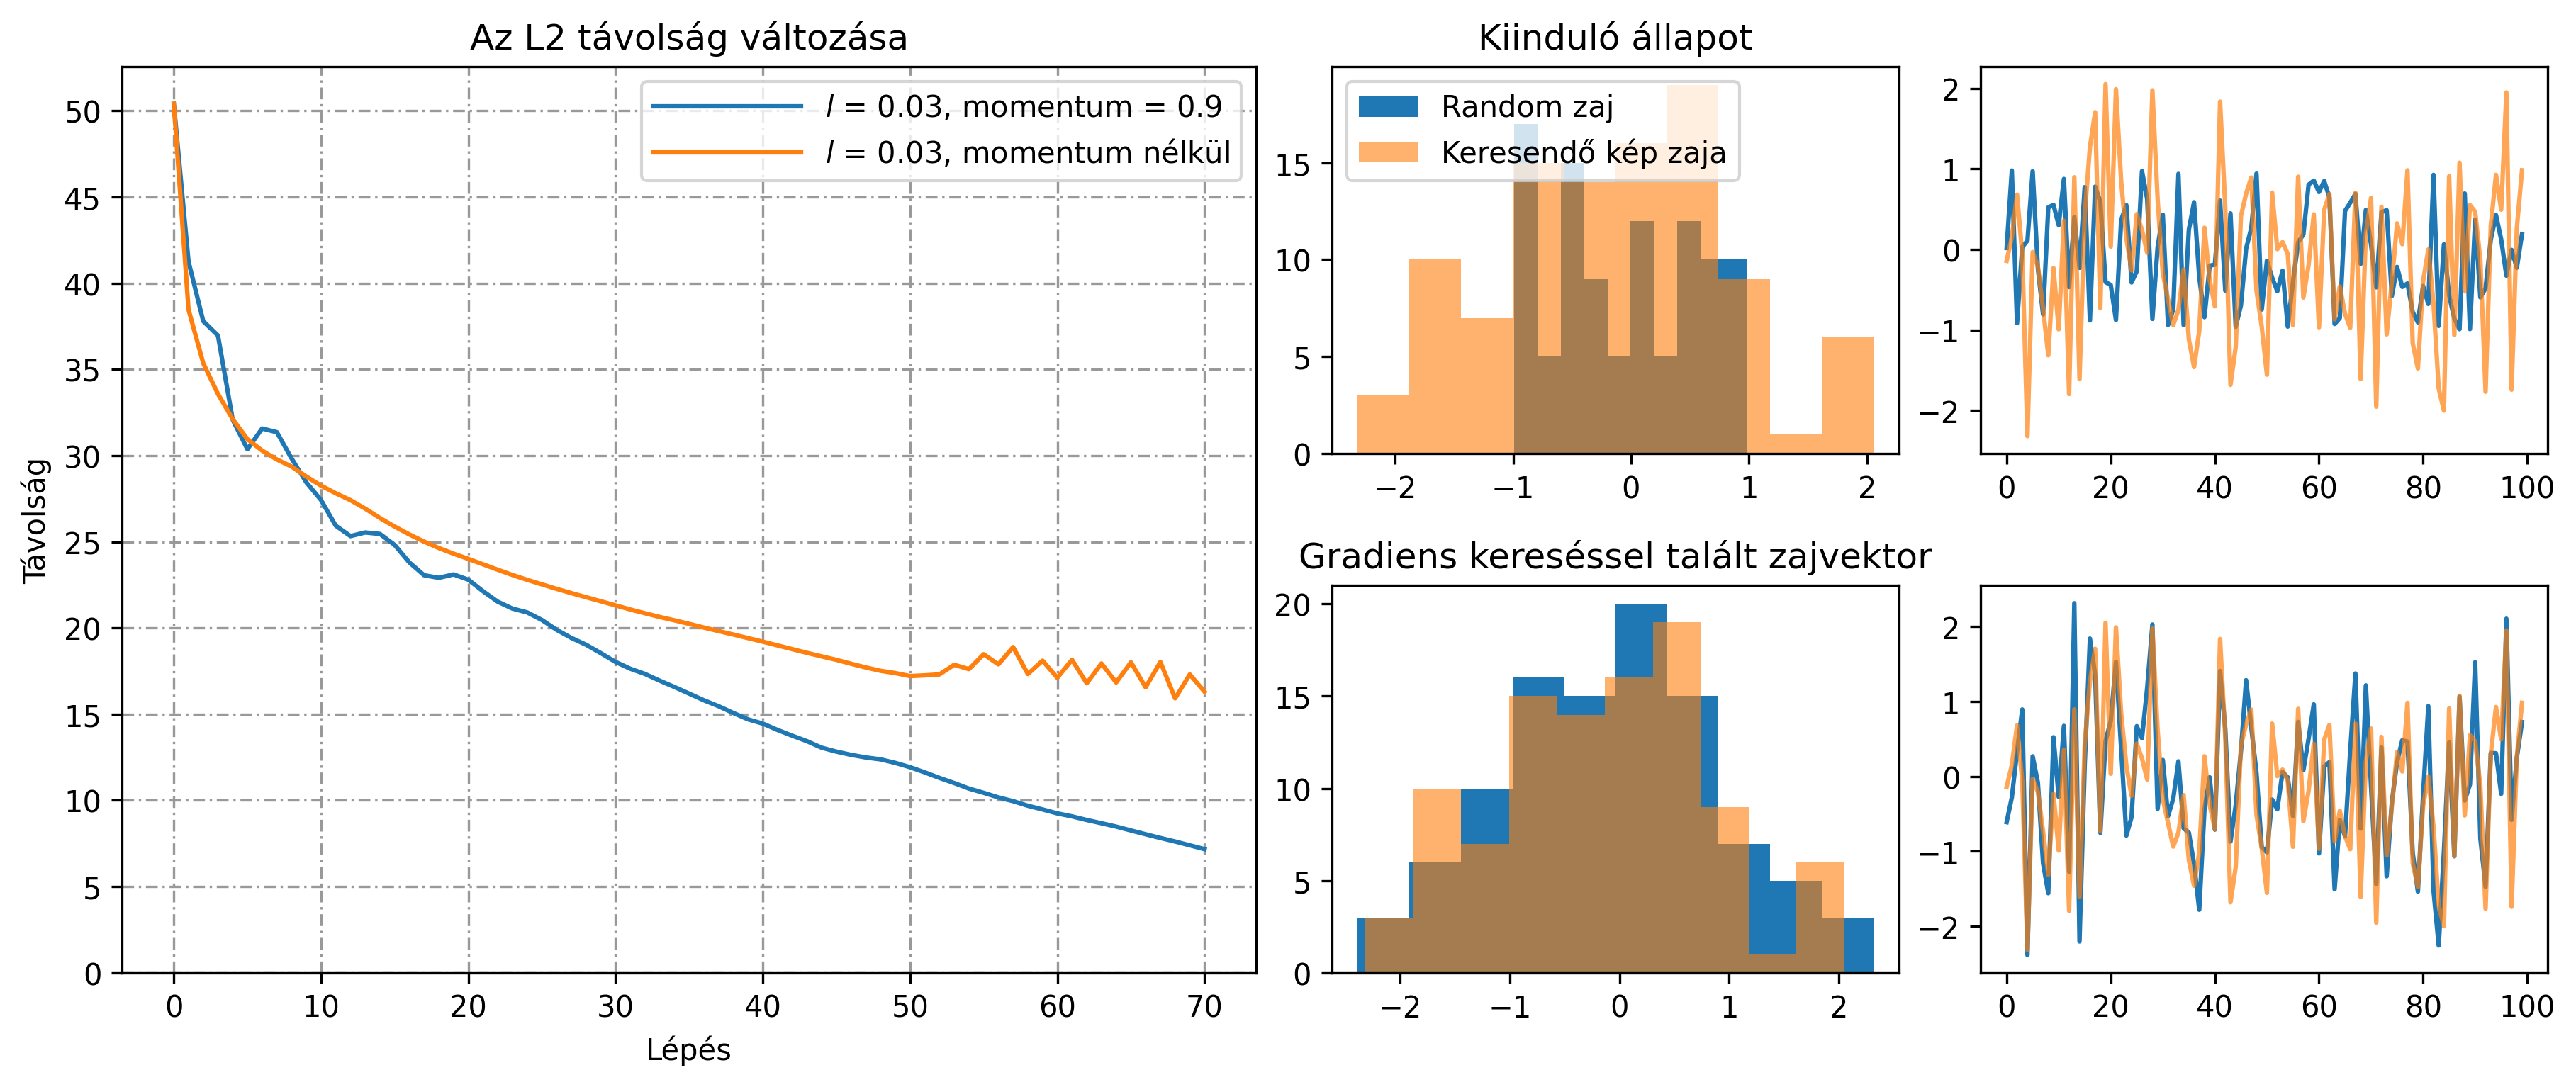
\includegraphics[width=15cm]{images/grad_losses.png}
\caption{A hibafüggvény változása a lépések során}
\label{fig:gradlosses}
\end{figure}


\begin{figure}[h]
\centering
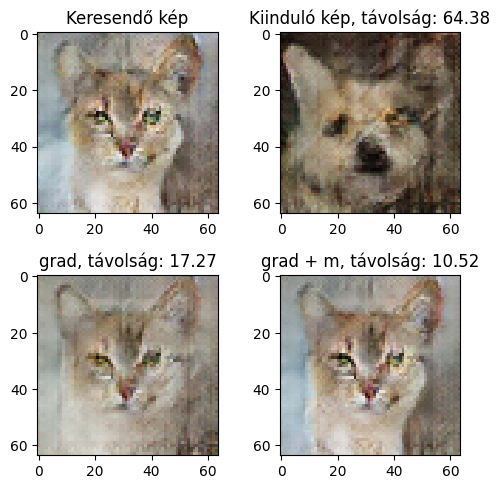
\includegraphics[width=8cm]{images/grad_found.png}
\caption{Gradiens kereséssel visszakeresett képek}
\label{fig:gradfound}
\end{figure}

\newpage

\Section{Képek keresése osztályozó segítségével}

A képek visszakeresése pixel szinten csupán azokban az esetekben adhat igazán jó megoldást, amikor a Generátor egy korábbi kimenetére végezzük el a keresést. Az előbbiekben erre láthattunk példát, a \ref{fig:gradfound} ábrán is az figyelhető meg, hogy a korábban kigenerált kép bemeneti vektorát hogyan sikerült a gradienslejtési módszerekkel (momentum nélkül és momentummal) visszakeresni.
Viszont ha egy külső forrásból érkező képet kívánunk így visszakeresni, akkor az eredményül kapott vektorból generált kép nem fogja olyan jól közelíteni a keresendő képet, hiába sikerült minimalizálnia a távolságot.
Ez értelemszerűen abból adódik, hogy az algoritmus a keresés során a nyers pixelértékeket veszi csupán csak figyelembe, a kép tartalmára tehát semmiféle információja nincsen. Viszont a Generátor nem képes minden pixelét egymástól függetlenül változtatni, hiszen a dekonvolúciós rétegeknek köszönhetően betanulta a tanítóhalmaz jellegzetességeit és a kigenerált képek is a tanítóhalmaz eloszlását követik. Így nem létezhet olyan bemeneti vektor, amellyel tetszőleges pixelértékeket felvehet a kimeneti kép.
Ha az eredeti adathalmazból  kívánunk képeket visszakeresni, akkor közelítő eredményeket kaphatunk, viszont ezek továbbra sem lesznek tökéletes találtatok, hiszen a GAN nem pixel pontosan tanulja be az adathalmaz elemeit, hanem azok jellegzetességeit tanulja meg reprezentálni, ezért is nevezik a GAN-t \textit{Representation-learning} \cite{geron2019hands} modellnek is.

Ha a hibafüggvényt kicseréljük és az optimalizációt egy, az adathalmazon tanított osztályozóval végezzük el, úgy viszonylag jó találatot kaphatunk. Természetesen ilyenkor az osztályozó teljesítményétől is függ az eredmény jósága.
Az irodalomkutatás során egyetlen munkát találtam, amely publikálva is volt (CLIPDRAW\cite{frans2021clipdraw}) a további ismertebb munkák csupán notebook-ok formájában érhetőek el. Viszont a közös bennük, hogy mind a CLIP\cite{radford2021learning} osztályozó kimenetei alapján végzik el az optimalizációt.

Egy hasonló megoldást alkalmaztam, viszont a CLIP osztályozó helyett egy saját modellt tanítottam be. Az betanított osztályozó modell alapja az Inception v3, amely a témám során több helyen is feltűnt, az IS és FID pontok számítás is ezen modellen alapszik. Az ImageNet \cite{deng2009imagenet} adatbázison tanított Inception modell az adatbázis 1000 darab osztályára képes osztályozni. Ha a modellt használni kívánjuk a saját osztályozónkba, akkor az úgynevezett \textit{Transfer-learning} technikát kell alkalmazni a tanításhoz, amelynek lényege, hogy egy, már betanított általános modellre egy újabb modellt építünk, amely egy szűkebb, speciális feladat megoldására szánunk. Esetünkben nincs szükség 1000 darab osztályra. Viszont az Inception modell-t felhasználhatjuk a képek jellegeinek kinyerésére és a modell utolsó rétegét pedig kicseréljük a saját osztályozónkra.
A tanítás során az eredeti modell súlyait lefagyasztjuk, vagyis a háló ezen részének paramétereit taníthatatlanná tesszük és a tanítás során csak az általunk hozzáadott rétegeket frissítjük.
A hibafüggvény számoláshoz a Kategórikus Kereszt-entrópiát (Categorical Cross-Entropy) használjuk fel. Az osztályozó modell tanítása ezek után a teljesen megszokott módon történik.

Az alábbi kódrészletben az osztályozó modell implementációja figyelhető meg.

\begin{python}
inputs = keras.Input(shape=(64, 64, 3))
x = data_augmentation(inputs)
resized = tf.image.resize(
    x, [299, 299],
    preserve_aspect_ratio=True, method='nearest'
)
x = inception_model(resized, training=False)
x = keras.layers.GlobalAveragePooling2D()(x)
x = keras.layers.Dropout(0.2)(x)
x = keras.layers.Dense(3)(x)
outputs = keras.layers.Activation("softmax")(x)
model = keras.Model(inputs, outputs)
\end{python}

Az újonnan kialakított modell bemenete megegyezik a betanított Generátor kimenetével. Az overfitting elkerülése érdekében, és hogy a modell ne az egyes számára érdekes pixelértékek alapján hozza meg a döntést, a bemenetre data augmentation technika kerül alkalmazásra, amely random minimális transzformációkat alkalmaz a bemenetre. A bemeneti képeket véletlenszerűen függőlegesen tükrözi, és random elforgatást alkalmaz. A Cifar-10 adathalmaz esetében úgy figyeltem meg, hogy az augmentation technika csak megnehezíti a konvergenciát és a modell nagyon sokat tévedett ennek hatására. A technika kihagyásával a tanítás jobb eredményt hozott, viszont ezen adathalmaz sokkal több tanítómintával rendelkezik, mint az AFHQ és a benne található képek is változatosabbak, így esetében lehetséges, hogy valóban nem indokolt a technika használata.

Az \texttt{inception\_model} a kódrészletben a már említett, csonkított változata az eredetinek. Az utolsó \texttt{Dense} rétegétől megfosztott változata, a lefagyasztott súlyokkal. Az Inception modell bemenetként $299 \times 299$ felbontású képet vár, így a képünket fel kell nagyítani a kívánt felbontásra. A nagyításhoz nearest interpolációt alkalmaztam, hogy a felbontás növelése ne járjon homályossággal, ugyanis azt figyeltem meg, hogy olyankor a modell gyengébben teljesít. (Ezt is le lehetne mérni?)
A csonkított Inception modell Kimenete egy (8, 8, 2048) alakú tensor, amely a bemeneti képekből kinyert feature-öket tartalmazza. A \texttt{GlobalAveragePooling2D} réteg az előbbi kimenetből 2048 elemű vektort készít, amelyet beadhatunk az utolsó \texttt{Dense} rétegnek, amely az osztályozást végzi el. Egy regularizációs technikaként, hogy csökkentsük az overfitting esélyét, egy \texttt{Dropout} réteg is helyet kapott a teljesen összekapcsolt réteg előtt.
A kimenetet \texttt{softmax} aktivációs függvénnyel normalizáljuk, így a modell használata során kimenetként megkapjuk az egyes osztályokhoz tartozó valószínűségi értékeket.

A kapott modellnek összesen 21 808 931 darab paramétere van, melyből csupán 6147 a tanítható paraméter. A tanítás során tehát az osztályozásért felelős rétegeket kell frissítenünk.

\begin{figure}[h]
	\centering
	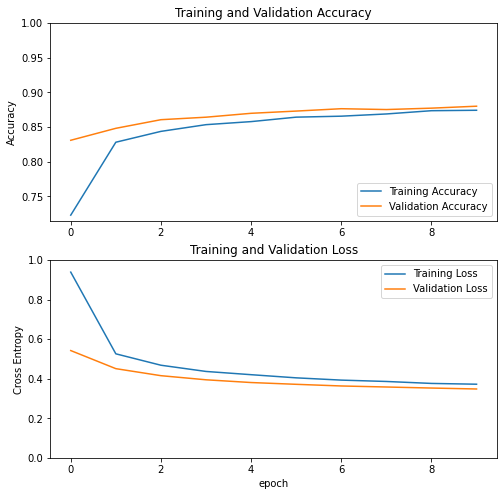
\includegraphics[width=8cm]{images/transfer_inception.png}
	\caption{Transfer-learning loss ábra (Inception modell)}
	\label{fig:transfer_learning_loss}
\end{figure}

Az optimaizálást a GAN tanításánál is használt Adam optimalizálóval végeztem, 0.0001 \textit{learning-rate} paraméterrel. A bemeneti dataset-et 32 elemű mini-batch-okra osztottam fel. A tanítást mindösszesen 10 epoch-ig futtattam. A nagy tanítóminta és a kevés tanítható paraméter miatt úgy figyeltem meg, hogy elegendő ennyi tanítás is. A konvergenciagörbe a Cifar-10 datasetre tanítva a \ref{fig:transfer_learning_loss} ábrán figyelhető meg.

%TODO: Confusion matrix melléklése!

Mivel a GAN tanítása után a Diszkriminátort elhagyjuk és további szerepe nincsen, úgy gondoltam, hogy akár hasonló módon is felhasználásra kerülhet, mint az előbbiekben ismertetett Inception modell. A tanulás során természetesen nem csupán a tanítóhalmazt látta a Diszkriminátor, hanem a generált képeket is, így elég specifikus tudással rendelkezik csupán. A háló súlyai úgy lettek optimalizálva, hogy belső reprezentációt állítson elő, amellyel a bináris osztályozást megfelelően el tudja végezni. Így a háló által kinyert jellegvektorok is oly módon állnak össze, hogy el tudja az alapján dönteni, hogy a kép valódi vagy hamis. A tanítást elvégeztem, viszont az így kapott összeállított új modell teljesítménye alulmaradt az Inception-t használó másik modellel szemben. A konvergencia görbe a \ref{fig:transfer_learning_loss_discriminator} ábrán figyelhető meg.

\begin{figure}[h]
	\centering
	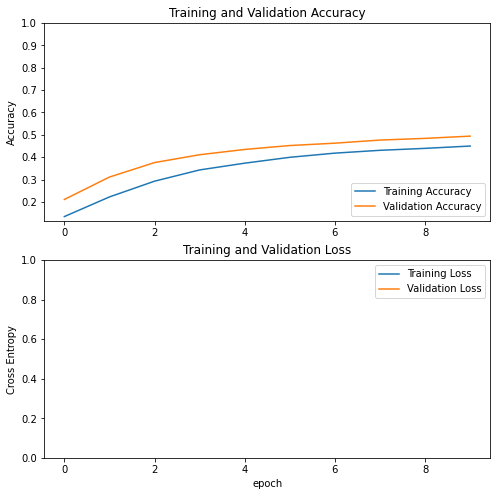
\includegraphics[width=8cm]{images/transfer_discriminator.png}
	\caption{Transfer-learning loss ábra (Inception modell)}
	\label{fig:transfer_learning_loss_discriminator}
\end{figure}

A bemeneti vektorok visszakeresése pedig a már ismertetett gradiens süllyesztés módszerrel valósul meg, viszont a hibafüggvény számolása a Kategórikus Kereszt-entrópia által kerül meghatározásra, hasonlóan, mint az osztályozó tanításánál. Az algoritmus bemenete tehát a kezdeti zajvektor, a keresendő címke és a gradiens módszer paraméterei (a lépésköz, a momentum és az iterációszám).
A bemeneti címkét \textit{One-Hot} enkódolással kell megadni a keresztentrópia számoláshoz, ugyanis az új osztályozó modell kimenete az adott osztályok valószínűségi értékei lesznek. A gradiens kereséssel pedig a keresztentrópia értéket kívánjuk csökkenteni. Tehát ha egy adott osztályra kívánunk egy olyan vektort kapni, amelyből a megfelelő osztályba tartozó képet ki tudja generálni a generátor, akkor ebben az esetben az osztályhoz tartozó valószínűségi érték 1 lesz, a többi osztályé pedig 0.
Amennyiben kevert osztályra kívánunk képet generálni, úgy olyan keresendő one-hot enkódolást kell megadnunk, amelyben a kívánt osztályok megfelelő súlyokkal rendelkeznek. Mivel a GAN tere folytonosan van kitöltve, így feltehető, hogy létezik olyan pont a térben, amely egyszerre több osztály jellegzetességeit is magában hordozza. A \ref{fig:interpolation} ábrán is megfigyelhető, hogy az interpoláció mintavételezett pontjaiban a két végpont között milyen folytonos az átmenet és a köztes állapotokban mindkét pont tulajdonságai megjelennek.

%TODO: A keresés optimélis paraméterei...

\begin{figure}[h]
	\centering
	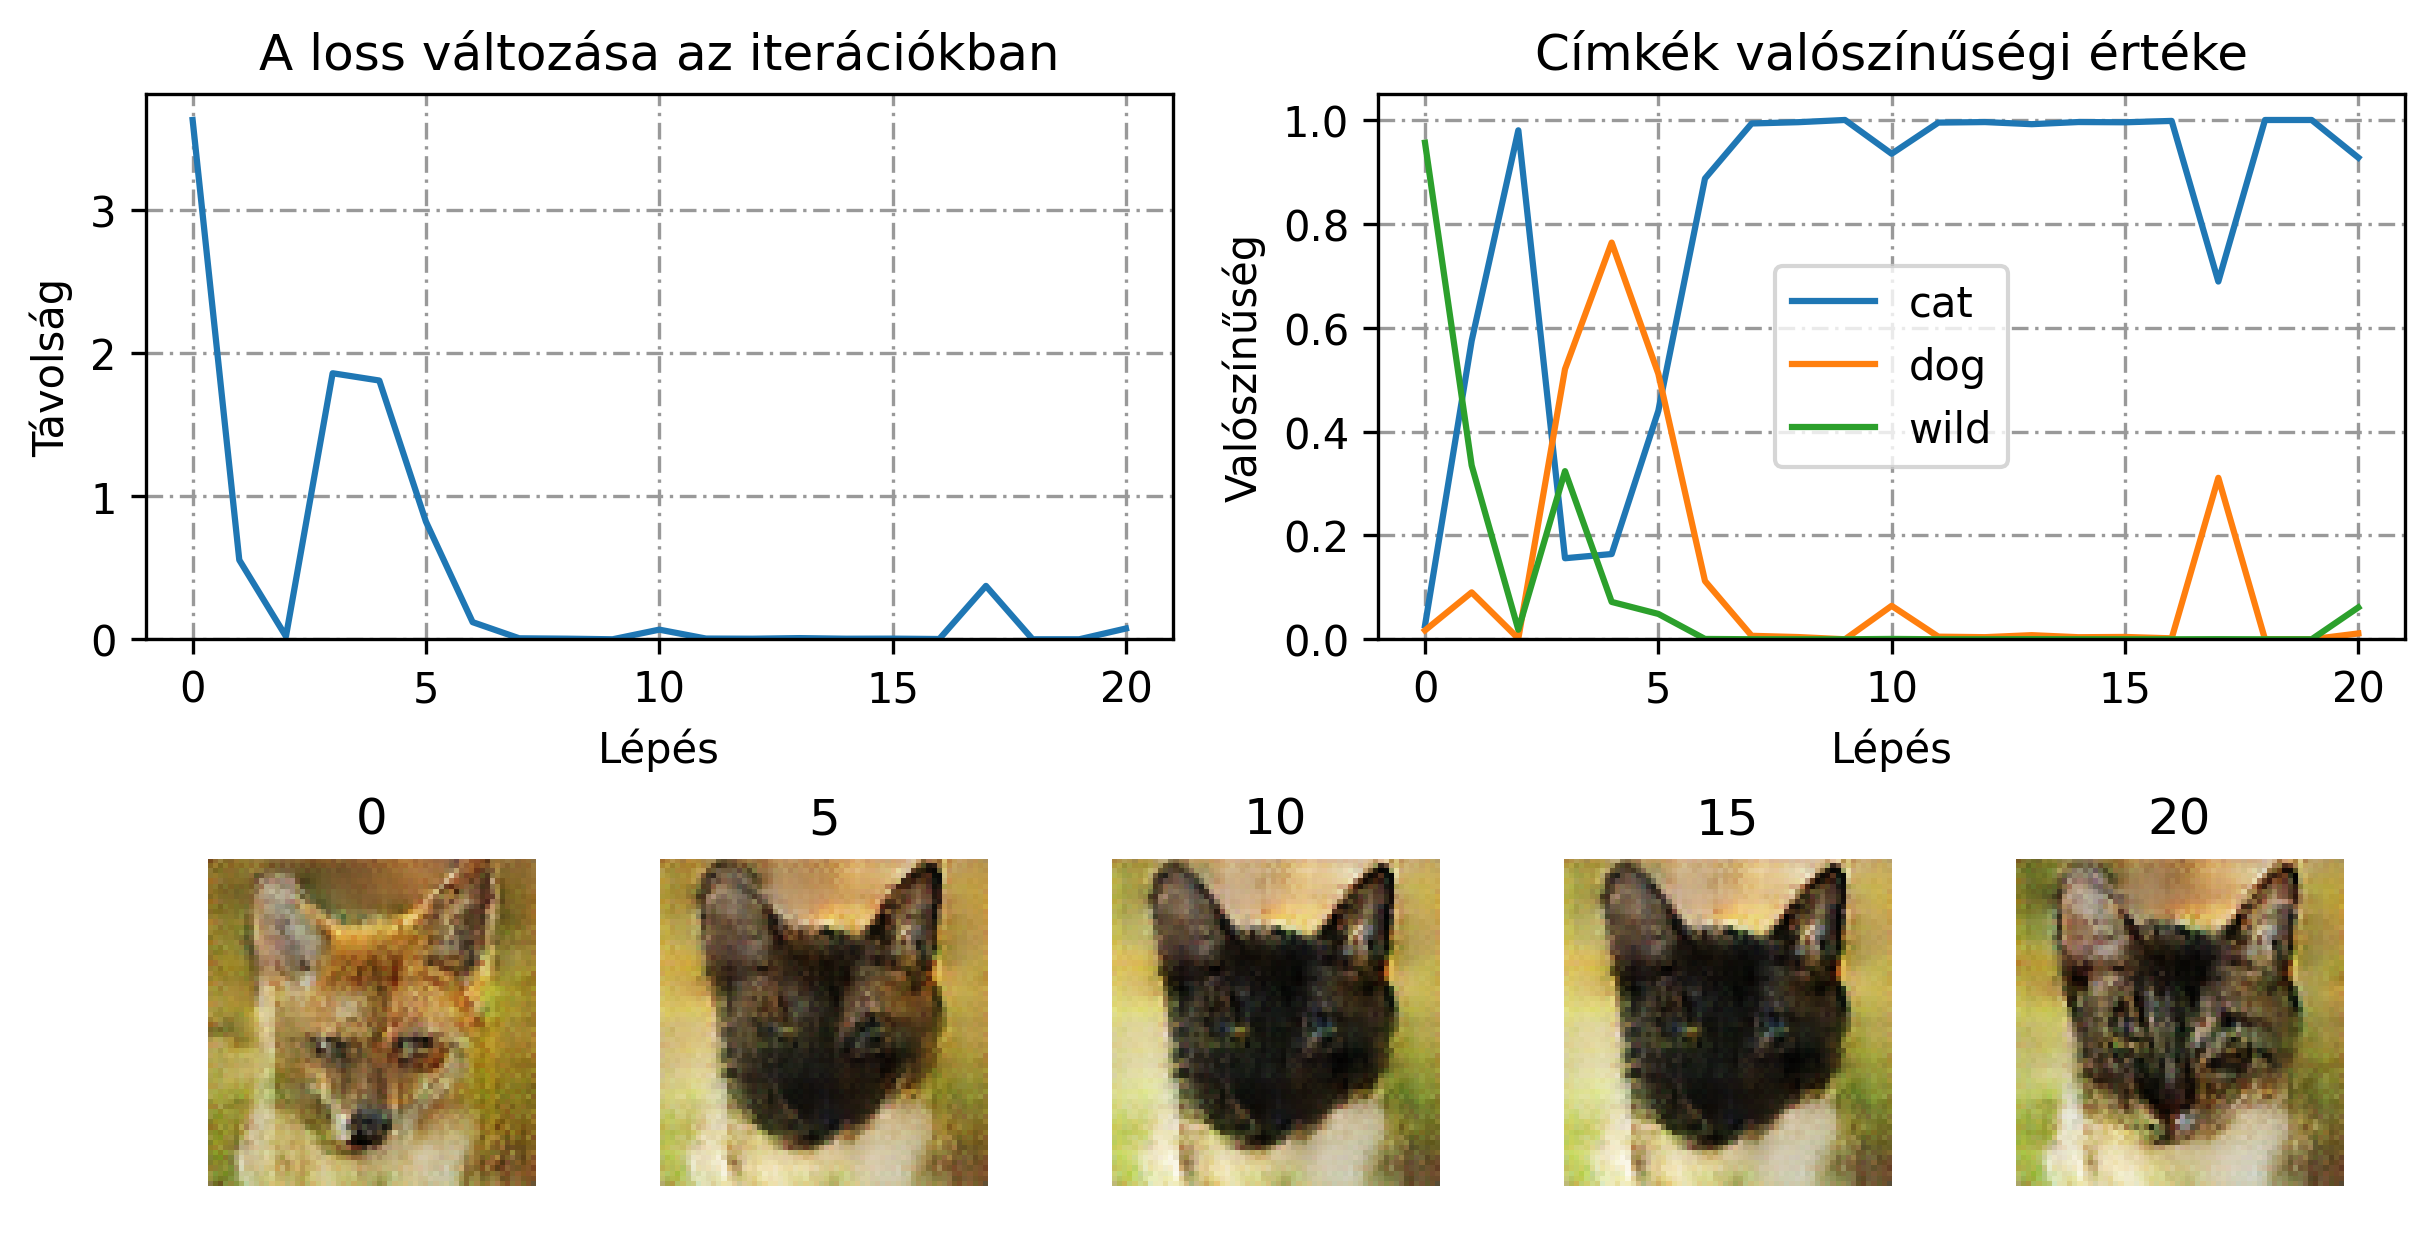
\includegraphics[width=15cm]{images/searching-cat.png}
	\caption{Kép generálása osztály szerint (Macska címkével)}
	\label{fig:searching}
\end{figure}

\begin{figure}[h]
	\centering
	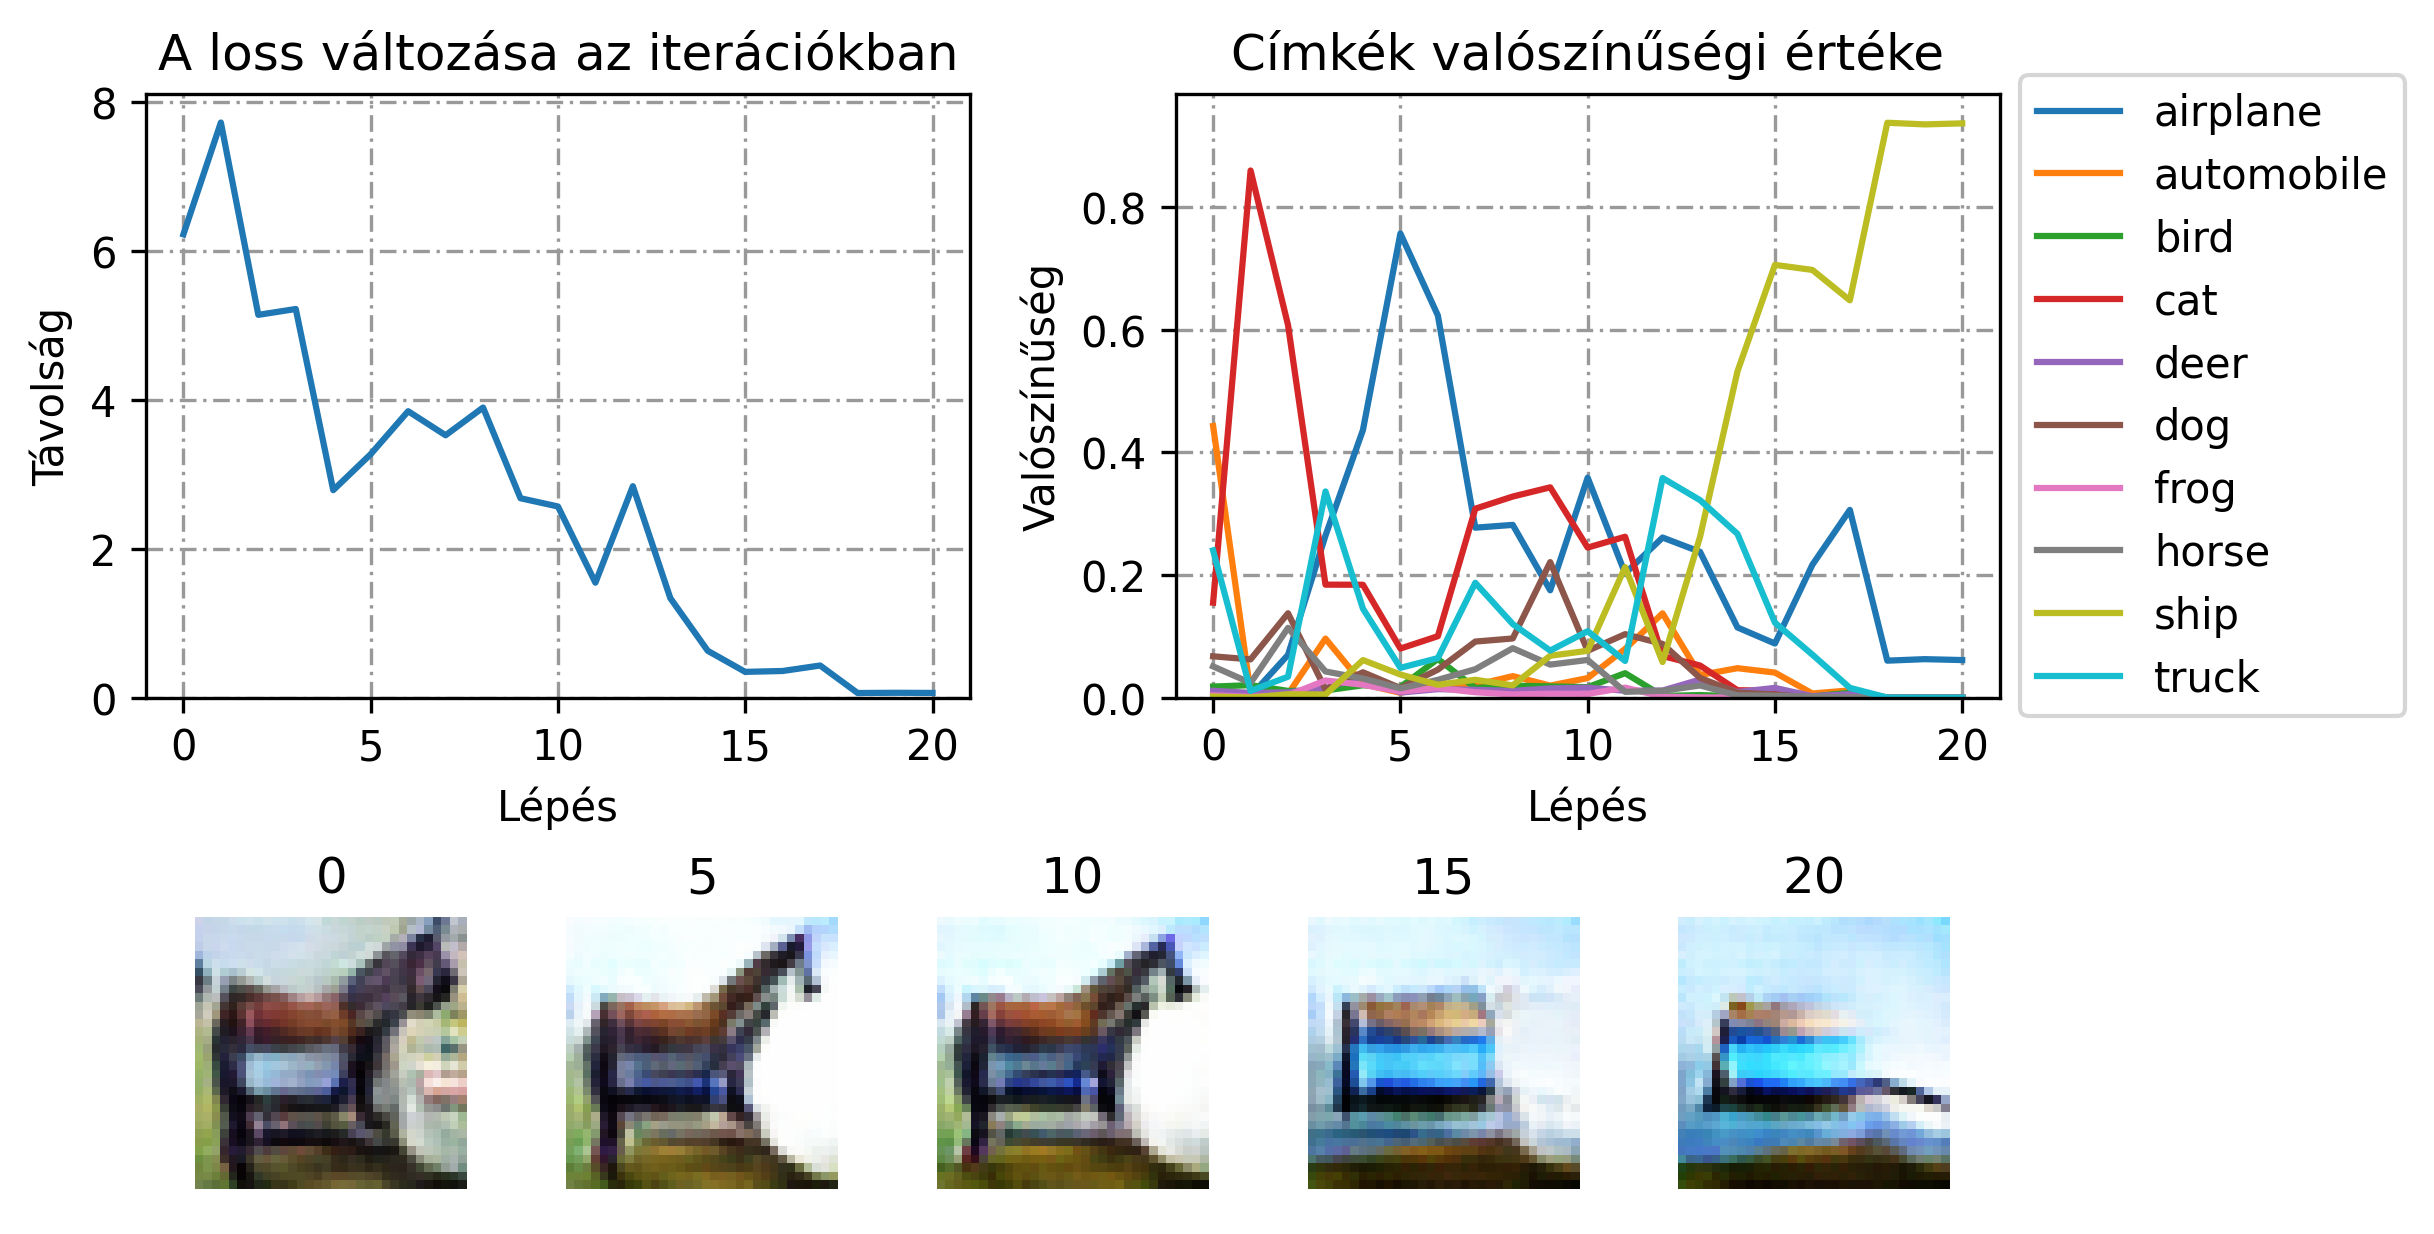
\includegraphics[width=15cm]{images/searching-cifar_ship.png}
	\caption{Kép generálása osztály szerint (Hajó címkével)}
	\label{fig:searching_ship}
\end{figure}
